\documentclass[11pt,a4paper]{article}
\usepackage[utf8]{inputenc}
\usepackage[T1]{fontenc}
\usepackage{geometry}
\usepackage{graphicx}
\usepackage{hyperref}
\usepackage{listings}
\usepackage{xcolor}
\usepackage{tikz}
\usepackage{pgfplots}
\usetikzlibrary{shapes,arrows,positioning,fit,backgrounds}
\usepackage{float}
\usepackage{booktabs}
\usepackage{longtable}
\usepackage{enumitem}
\usepackage{amsmath}
\usepackage{amssymb}
\usepackage{adjustbox}

% Page setup
\geometry{margin=2.5cm}
\hypersetup{
    colorlinks=true,
    linkcolor=blue,
    filecolor=magenta,      
    urlcolor=cyan,
    pdftitle={Uptimatum Documentation},
    pdfauthor={Uptimatum Project},
    pdfsubject={Complete Documentation for Uptimatum Status Page Platform}
}

% Code listing style
\lstset{
    basicstyle=\ttfamily\small,
    breaklines=true,
    frame=single,
    numbers=left,
    numberstyle=\tiny\color{gray},
    keywordstyle=\color{blue},
    commentstyle=\color{green!60!black},
    stringstyle=\color{red},
    backgroundcolor=\color{gray!10}
}

% Title
\title{\textbf{Uptimatum}\\
\large The Ultimate Self-Hosted Status Page Platform\\
\large Complete Documentation}
\author{Uptimatum Project}
\date{\today}

\begin{document}

\maketitle

\begin{abstract}
Uptimatum is a complete Kubernetes-based microservices application for monitoring endpoint uptime with real-time status pages, embeddable badges, and beautiful dashboards. This document provides comprehensive documentation covering architecture, deployment, development, and usage of the platform.
\end{abstract}

\tableofcontents
\newpage
\listoffigures
\newpage

\section{Introduction}

Uptimatum is a self-hosted status page platform designed to monitor endpoint uptime with real-time status updates. The system is built as a microservices application running on Kubernetes, featuring a modern web frontend, RESTful API backend, and a highly available PostgreSQL database cluster.

\subsection{Key Features}

\begin{itemize}
    \item Multi-endpoint monitoring with real-time status updates
    \item 24-hour uptime percentage calculation
    \item Response time metrics tracking
    \item Status timeline visualization
    \item Incident management for service outages
    \item Beautiful, customizable status pages
    \item Public-facing status pages
    \item Embeddable widgets and SVG badges
    \item Dark mode support
    \item Mobile responsive design
    \item Optimized database writes (only inserts when status changes)
\end{itemize}

\subsection{Technology Stack}

\begin{itemize}
    \item \textbf{Frontend}: SolidJS, TypeScript, TailwindCSS
    \item \textbf{Backend}: Hono, Bun, Drizzle ORM
    \item \textbf{Database}: PostgreSQL HA (Bitnami Helm chart with StatefulSets)
    \item \textbf{Infrastructure}: Google Kubernetes Engine (GKE)
    \item \textbf{Container Registry}: Google Artifact Registry
\end{itemize}

\section{Architecture}
\subsection{System Architecture}

The Uptimatum system follows a microservices architecture deployed on Google Kubernetes Engine. The architecture consists of multiple layers:

\begin{figure}[H]
\centering
\begin{adjustbox}{max width=\textwidth,center,angle=0}
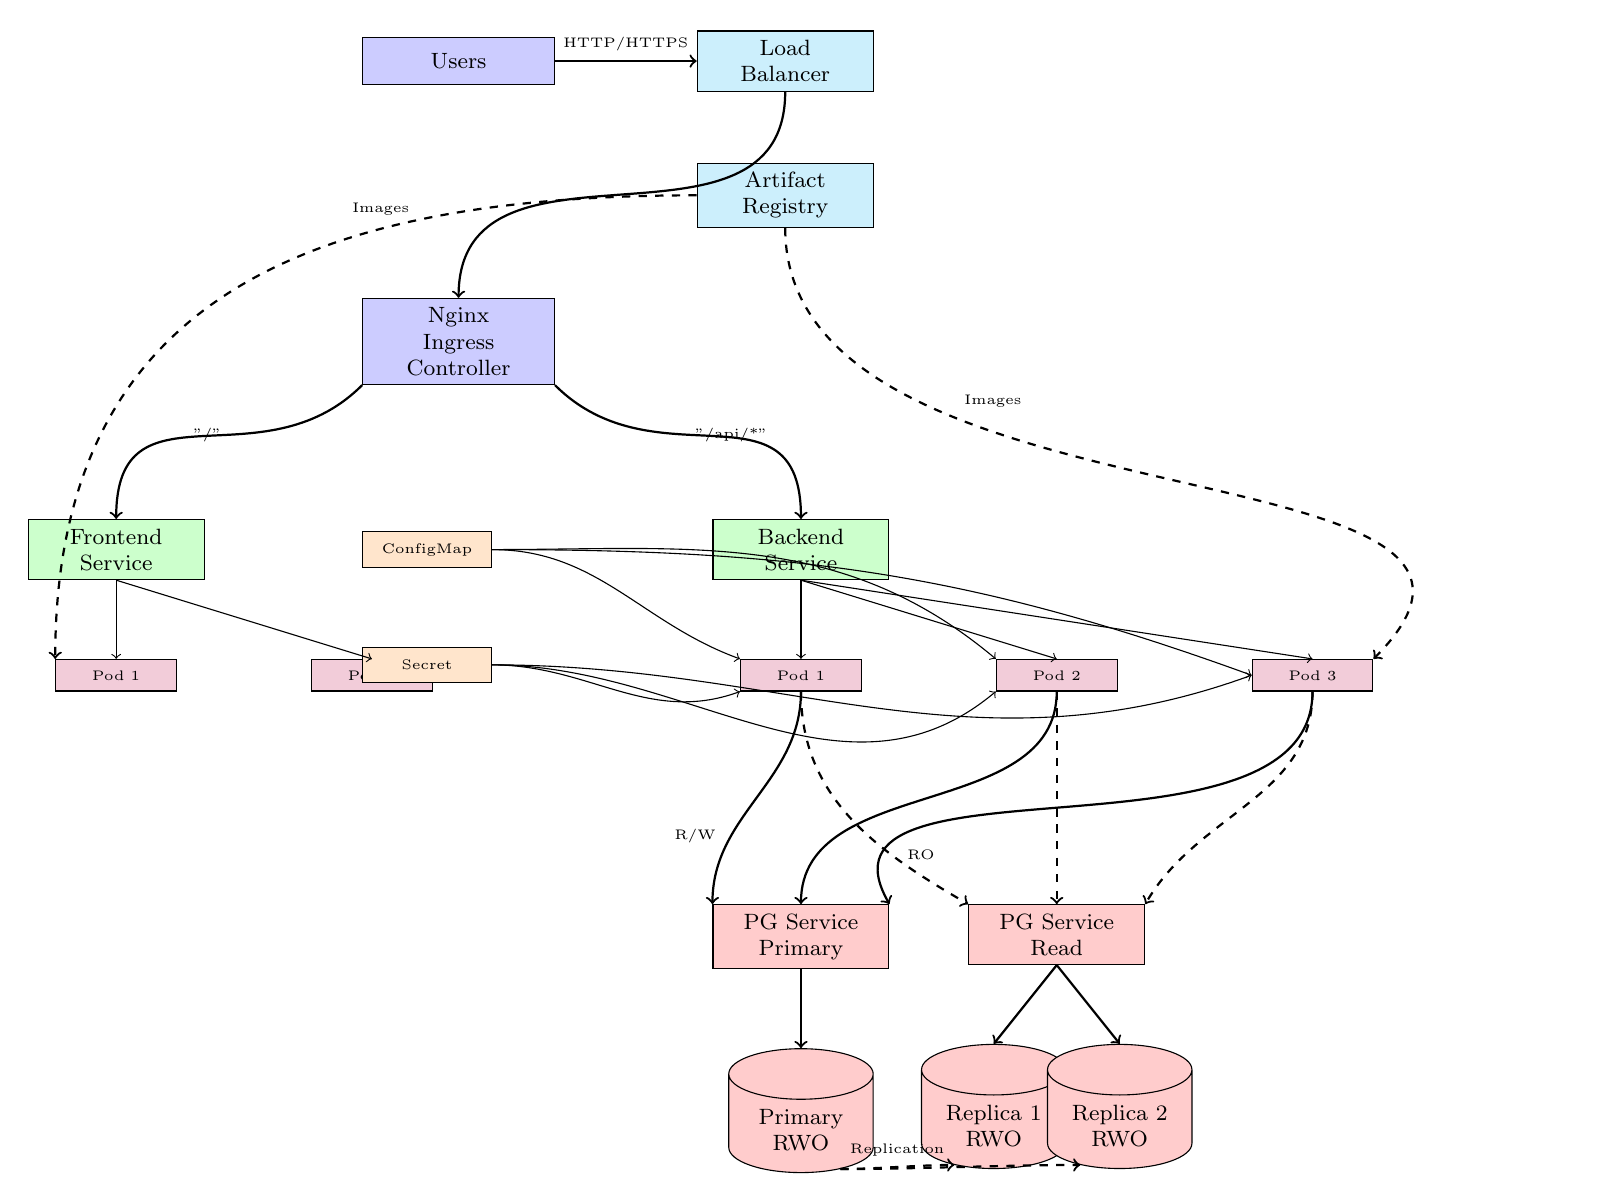
\begin{tikzpicture}[
    node distance=1.2cm and 1.5cm,
    box/.style={rectangle, draw, fill=blue!20, text width=2.2cm, text centered, minimum height=0.6cm, font=\footnotesize},
    service/.style={rectangle, draw, fill=green!20, text width=2cm, text centered, minimum height=0.55cm, font=\footnotesize},
    pod/.style={rectangle, draw, fill=purple!20, text width=1.3cm, text centered, minimum height=0.4cm, font=\tiny},
    db/.style={cylinder, draw, fill=red!20, text width=1.6cm, text centered, minimum height=0.6cm, shape border rotate=90, aspect=0.35, font=\footnotesize},
    db-service/.style={rectangle, draw, fill=red!20, text width=2cm, text centered, minimum height=0.55cm, font=\footnotesize},
    config/.style={rectangle, draw, fill=orange!20, text width=1.4cm, text centered, minimum height=0.45cm, font=\tiny},
    gcp/.style={rectangle, draw, fill=cyan!20, text width=2cm, text centered, minimum height=0.55cm, font=\footnotesize}
]

% Internet layer - centered
\node[box] (user) at (0,0) {Users};

% GCP Services layer
\node[gcp, right=of user, xshift=0.3cm] (lb) {Load\\Balancer};
\node[gcp, below=of lb, yshift=0.3cm] (artifact) {Artifact\\Registry};

% Ingress layer
\node[box, below=of user, yshift=-1.5cm] (ingress) {Nginx\\Ingress\\Controller};

% Application layer - Frontend (left side)
\node[service, below left=of ingress, xshift=-0.5cm, yshift=-0.5cm] (fe-svc) {Frontend\\Service};
\node[pod, below=of fe-svc, yshift=0.2cm] (fe1) {Pod 1};
\node[pod, right=of fe1, xshift=0.2cm] (fe2) {Pod 2};

% Application layer - Backend (right side)
\node[service, below right=of ingress, xshift=0.5cm, yshift=-0.5cm] (be-svc) {Backend\\Service};
\node[pod, below=of be-svc, yshift=0.2cm] (be1) {Pod 1};
\node[pod, right=of be1, xshift=0.2cm] (be2) {Pod 2};
\node[pod, right=of be2, xshift=0.2cm] (be3) {Pod 3};

% Configuration (left of backend)
\node[config, left=of be-svc, xshift=-1.3cm] (configmap) {ConfigMap};
\node[config, below=of configmap, yshift=0.2cm] (secret) {Secret};

% Data layer - Services (below backend pods with more space)
\node[db-service, below=of be1, yshift=-1.5cm] (pg-svc) {PG Service\\Primary};
\node[db-service, below=of be2, yshift=-1.5cm] (pg-read-svc) {PG Service\\Read};

% Data layer - StatefulSets (below services)
\node[db, below=of pg-svc, yshift=0.2cm] (pg-primary) {Primary\\RWO};
\node[db, below=of pg-read-svc, xshift=-0.8cm, yshift=0.2cm] (pg-replica1) {Replica 1\\RWO};
\node[db, below=of pg-read-svc, xshift=0.8cm, yshift=0.2cm] (pg-replica2) {Replica 2\\RWO};

% Connections - Internet to GCP
\draw[->, thick] (user.east) -- node[above, font=\tiny] {HTTP/HTTPS} (lb.west);

% Connections - GCP to Ingress
\draw[->, thick] (lb.south) to[out=270,in=90, looseness=1.2] (ingress.north);

% Connections - Ingress to Services
\draw[->, thick] (ingress.south west) to[out=225,in=90, looseness=1.3] node[left, font=\tiny, pos=0.4] {"/"} (fe-svc.north);
\draw[->, thick] (ingress.south east) to[out=315,in=90, looseness=1.3] node[right, font=\tiny, pos=0.4] {"/api/*"} (be-svc.north);

% Connections - Services to Pods
\draw[->] (fe-svc.south) -- (fe1.north);
\draw[->] (fe-svc.south) -- (fe2.north);
\draw[->] (be-svc.south) -- (be1.north);
\draw[->] (be-svc.south) -- (be2.north);
\draw[->] (be-svc.south) -- (be3.north);

% Connections - Backend Pods to Primary DB Service (using side anchors to spread out)
\draw[->, thick] (be1.south) to[out=270,in=90] node[left, font=\tiny, pos=0.7, xshift=-2pt] {R/W} (pg-svc.north west);
\draw[->, thick] (be2.south) to[out=270,in=90] (pg-svc.north);
\draw[->, thick] (be3.south) to[out=270,in=120] (pg-svc.north east);

% Connections - Backend Pods to Read Replica Service (using side anchors)
\draw[dashed,->, thick] (be1.south) to[out=270,in=150] node[right, font=\tiny, pos=0.7, xshift=2pt] {RO} (pg-read-svc.north west);
\draw[dashed,->, thick] (be2.south) to[out=270,in=90] (pg-read-svc.north);
\draw[dashed,->, thick] (be3.south) to[out=270,in=60] (pg-read-svc.north east);

% Connections - Database Services to StatefulSets
\draw[->, thick] (pg-svc.south) -- (pg-primary.north);
\draw[->, thick] (pg-read-svc.south) -- (pg-replica1.north);
\draw[->, thick] (pg-read-svc.south) -- (pg-replica2.north);

% Connections - Primary to Replicas (Streaming Replication)
\draw[dashed,->, thick] (pg-primary.south east) to[out=0,in=180, looseness=0.8] node[above, font=\tiny, pos=0.5] {Replication} (pg-replica1.south west);
\draw[dashed,->, thick] (pg-primary.south east) to[out=0,in=180, looseness=0.8] (pg-replica2.south west);

% Connections - Configuration to Backend Pods (using top anchors to avoid overlap)
\draw[->] (configmap.east) to[out=0,in=160] (be1.north west);
\draw[->] (configmap.east) to[out=0,in=140] (be2.north west);
\draw[->] (configmap.east) to[out=0,in=160] (be3.west);
\draw[->] (secret.east) to[out=0,in=200] (be1.south west);
\draw[->] (secret.east) to[out=0,in=220] (be2.south west);
\draw[->] (secret.east) to[out=0,in=200] (be3.west);

% Connections - Artifact Registry to Pods (going around the sides)
\draw[dashed,->, thick] (artifact.west) to[out=180,in=90, looseness=1.2] node[above, font=\tiny, pos=0.3, xshift=-5pt] {Images} (fe1.north west);
\draw[dashed,->, thick] (artifact.south) to[out=270,in=45, looseness=1.1] node[above right, font=\tiny, pos=0.3] {Images} (be3.north east);

\end{tikzpicture}
\end{adjustbox}
\caption{System Architecture Overview}
\end{figure}

\subsection{Backend Project Technologies}

\begin{figure}[H]
\centering
\includegraphics[width=0.8\textwidth]{../diagrams/uptimatum-backend.png}
\caption{Backend Project Technology Stack}
\end{figure}

The backend is built using:
\begin{itemize}
    \item \textbf{Hono}: Fast web framework with OpenAPI support
    \item \textbf{Bun}: High-performance JavaScript runtime
    \item \textbf{Drizzle ORM}: Type-safe SQL ORM
    \item \textbf{Zod}: Schema validation
    \item \textbf{Pino}: Structured logging
    \item \textbf{node-cron}: Scheduled health checks
\end{itemize}

\subsection{Frontend Project Technologies}

\begin{figure}[H]
\centering
\includegraphics[width=0.8\textwidth]{../diagrams/uptimatum-frontend.png}
\caption{Frontend Project Technology Stack}
\end{figure}

The frontend is built using:
\begin{itemize}
    \item \textbf{SolidJS}: Reactive UI framework
    \item \textbf{TypeScript}: Type-safe development
    \item \textbf{TailwindCSS}: Utility-first CSS framework
    \item \textbf{Solid Router}: Client-side routing
    \item \textbf{Vite}: Build tool and dev server
\end{itemize}

\subsection{Database Schema}

\begin{figure}[H]
\centering
\includegraphics[width=0.9\textwidth]{../diagrams/database_schema.png}
\caption{Database Entity Relationship Diagram}
\end{figure}

The database consists of four main tables:

\begin{description}
    \item[\textbf{pages}] Stores status page definitions with unique slugs
    \item[\textbf{endpoints}] Monitored endpoints associated with pages
    \item[\textbf{checks}] Health check results with status, response time, and timestamps
    \item[\textbf{incidents}] Service incidents and outage tracking
\end{description}

\subsection{Data Flow}

The system follows a request-response pattern with background health checking:

\begin{figure}[H]
\centering
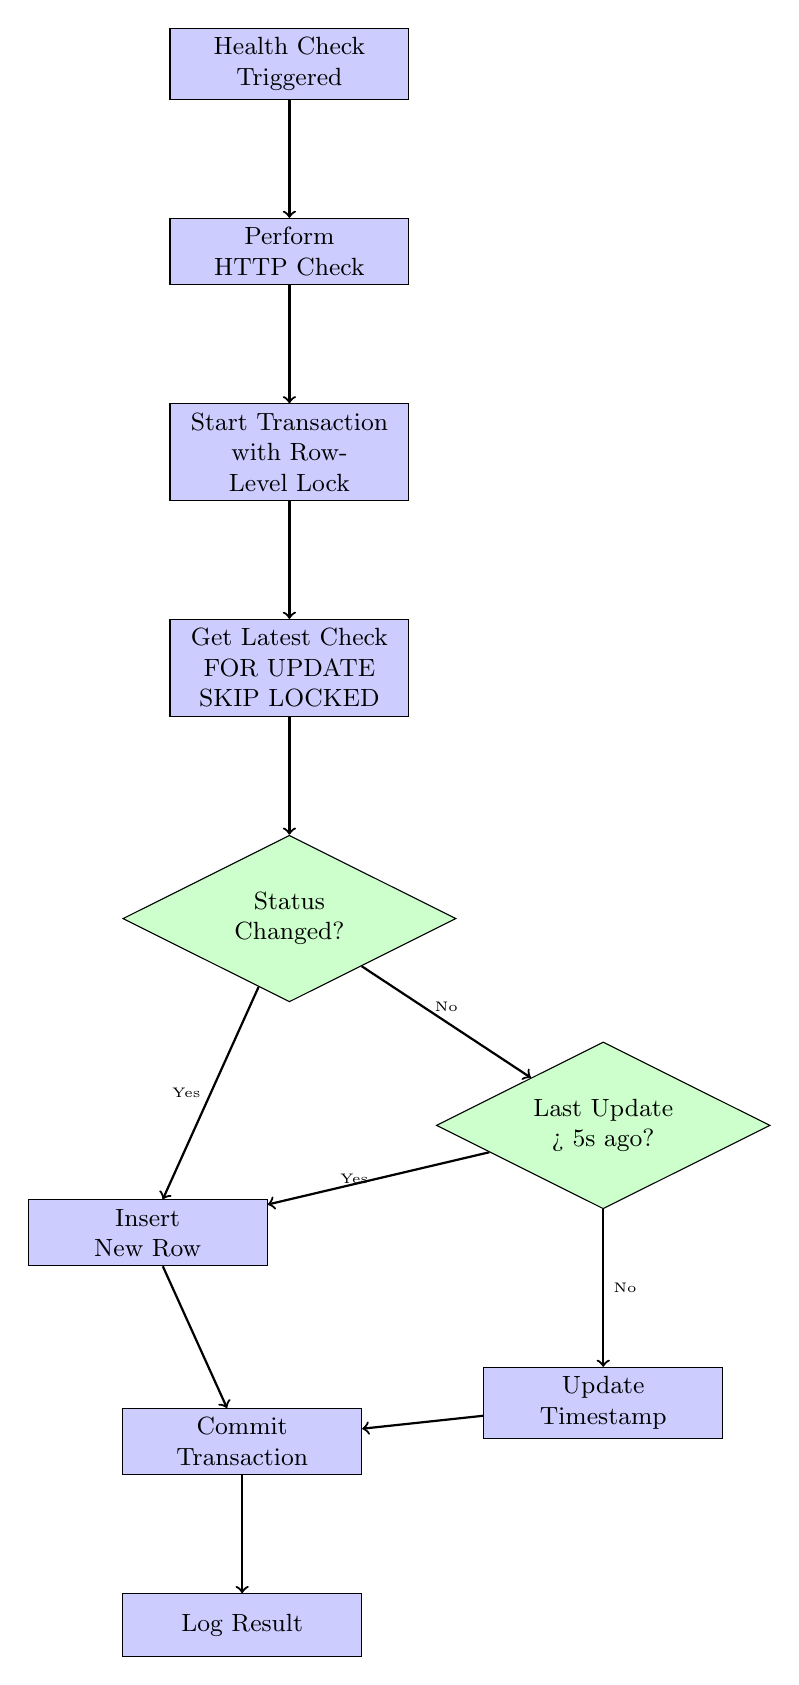
\begin{tikzpicture}[
    node distance=1.5cm,
    process/.style={rectangle, draw, fill=blue!20, text width=2.8cm, text centered, minimum height=0.8cm, font=\small},
    decision/.style={diamond, draw, fill=green!20, text width=2.2cm, text centered, aspect=2, font=\small}
]

% Health check flow
\node[process] (trigger) {Health Check\\Triggered};
\node[process, below=of trigger] (http) {Perform\\HTTP Check};
\node[process, below=of http] (tx) {Start Transaction\\with Row-Level Lock};
\node[process, below=of tx] (get) {Get Latest Check\\FOR UPDATE SKIP LOCKED};
\node[decision, below=of get] (status) {Status\\Changed?};
\node[decision, below right=of status, xshift=0.8cm, yshift=-0.5cm] (threshold) {Last Update\\> 5s ago?};
\node[process, below=of status, xshift=-1.8cm, yshift=-1cm] (insert) {Insert\\New Row};
\node[process, below=of threshold, yshift=-0.5cm] (update) {Update\\Timestamp};
\node[process, below=of insert, xshift=1.2cm, yshift=-0.3cm] (commit) {Commit\\Transaction};
\node[process, below=of commit] (log) {Log Result};

% Connections
\draw[->, thick] (trigger) -- (http);
\draw[->, thick] (http) -- (tx);
\draw[->, thick] (tx) -- (get);
\draw[->, thick] (get) -- (status);
\draw[->, thick] (status) -- node[left, font=\tiny] {Yes} (insert);
\draw[->, thick] (status) -- node[above, font=\tiny] {No} (threshold);
\draw[->, thick] (threshold) -- node[left, font=\tiny] {Yes} (insert);
\draw[->, thick] (threshold) -- node[right, font=\tiny] {No} (update);
\draw[->, thick] (insert) -- (commit);
\draw[->, thick] (update) -- (commit);
\draw[->, thick] (commit) -- (log);

\end{tikzpicture}
\caption{Health Check Database Write Optimization Flow}
\end{figure}

\section{Deployment}

\subsection{Prerequisites}

Before deploying Uptimatum, ensure you have:

\begin{enumerate}
    \item Google Cloud Account with billing enabled
    \item \texttt{gcloud} CLI installed and configured
    \item \texttt{kubectl} installed
    \item \texttt{helm} installed
    \item \texttt{bun} installed (or use nvm + bun)
\end{enumerate}

\subsection{Quick Start (Automated)}

The fastest way to deploy Uptimatum is using the master setup script:

\begin{lstlisting}[language=bash]
./scripts/setup.sh
\end{lstlisting}

This script performs the following steps:
\begin{enumerate}
    \item Enables required GCP APIs
    \item Creates Artifact Registry
    \item Creates GKE cluster with autoscaling
    \item Installs Nginx Ingress Controller
    \item Sets up PostgreSQL HA cluster (3 nodes)
    \item Builds and deploys application
\end{enumerate}

\textbf{Time}: Approximately 15-20 minutes

\subsection{Step-by-Step Manual Setup}

\subsubsection{Step 1: Configure GCP Project}

\begin{lstlisting}[language=bash]
export PROJECT_ID=your-project-id
gcloud config set project $PROJECT_ID
gcloud config get-value project
\end{lstlisting}

\subsubsection{Step 2: Enable Required APIs}

\begin{lstlisting}[language=bash]
gcloud services enable container.googleapis.com
gcloud services enable artifactregistry.googleapis.com
\end{lstlisting}

\subsubsection{Step 3: Create Artifact Registry}

\begin{lstlisting}[language=bash]
export REGION=europe-west1
export REPO=uptimatum

gcloud artifacts repositories create $REPO \
  --repository-format=docker \
  --location=$REGION \
  --description="Uptimatum Docker images"

gcloud auth configure-docker ${REGION}-docker.pkg.dev
\end{lstlisting}

\subsubsection{Step 4: Create GKE Cluster}

\begin{lstlisting}[language=bash]
export ZONE=${REGION}-b

gcloud container clusters create uptimatum-cluster \
  --zone=$ZONE \
  --num-nodes=3 \
  --machine-type=e2-standard-2 \
  --enable-autoscaling \
  --min-nodes=3 \
  --max-nodes=6

gcloud container clusters get-credentials uptimatum-cluster --zone=$ZONE
\end{lstlisting}

\textbf{Note}: Cluster creation takes 5-10 minutes.

\subsubsection{Step 5: Install Nginx Ingress Controller}

\begin{lstlisting}[language=bash]
kubectl apply -f https://raw.githubusercontent.com/kubernetes/ingress-nginx/controller-v1.14.0/deploy/static/provider/cloud/deploy.yaml

kubectl wait --namespace ingress-nginx \
  --for=condition=ready pod \
  --selector=app.kubernetes.io/component=controller \
  --timeout=300s
\end{lstlisting}

\subsubsection{Step 6: Setup PostgreSQL Database}

\begin{lstlisting}[language=bash]
./scripts/setup-db.sh
\end{lstlisting}

This script:
\begin{itemize}
    \item Adds the Bitnami Helm repository
    \item Installs/upgrades PostgreSQL using Bitnami Helm chart
    \item Creates the \texttt{uptimatum} namespace
    \item Deploys PostgreSQL cluster with 1 primary + 2 read replicas using StatefulSets
    \item Waits for all pods to become ready
\end{itemize}

\textbf{Primary-Replica Architecture:}

Bitnami PostgreSQL Helm chart sets up a master-replica architecture using StatefulSets:
\begin{itemize}
    \item \textbf{1 Primary (Master) StatefulSet}: Handles all read-write operations with RWO storage
    \item \textbf{2 Read Replicas StatefulSet}: Read-only nodes that sync from primary via streaming replication with RWO storage
    \item \textbf{Services}:
    \begin{itemize}
        \item \texttt{uptimatum-db-postgresql-primary}: Points to PRIMARY (read-write) - used by backend
        \item \texttt{uptimatum-db-postgresql-read}: Points to READ REPLICAS (read-only) - for read scaling
    \end{itemize}
\end{itemize}

Each StatefulSet pod has its own PersistentVolumeClaim for data persistence.

\subsubsection{Step 7: Build and Deploy Application}

\begin{lstlisting}[language=bash]
./scripts/deploy.sh
\end{lstlisting}

This will:
\begin{itemize}
    \item Build backend Docker image
    \item Build frontend Docker image
    \item Push images to Artifact Registry
    \item Deploy to Kubernetes
\end{itemize}

\subsection{Verifying Deployment}

\subsubsection{Check Pods}

\begin{lstlisting}[language=bash]
kubectl get pods -n uptimatum
\end{lstlisting}

Expected output:
\begin{verbatim}
NAME                                    READY   STATUS    RESTARTS   AGE
backend-xxx                              1/1     Running   0          2m
frontend-xxx                             1/1     Running   0          2m
uptimatum-db-postgresql-primary-0        1/1     Running   0          5m
uptimatum-db-postgresql-read-0           1/1     Running   0          5m
uptimatum-db-postgresql-read-1           1/1     Running   0          5m
\end{verbatim}

\subsubsection{Check Services}

\begin{lstlisting}[language=bash]
kubectl get svc -n uptimatum
\end{lstlisting}

Expected services for database:
\begin{itemize}
    \item \texttt{uptimatum-db-postgresql-primary}: Read-write service (points to primary StatefulSet)
    \item \texttt{uptimatum-db-postgresql-read}: Read-only service (points to read replica StatefulSet)
\end{itemize}

\subsubsection{Verify Primary-Replica Setup}

\begin{lstlisting}[language=bash]
# Check StatefulSets
kubectl get statefulset -n uptimatum

# Check which pods belong to primary vs read replicas
kubectl get pods -n uptimatum -l app.kubernetes.io/name=postgresql -o wide

# Check PersistentVolumeClaims (one per StatefulSet pod)
kubectl get pvc -n uptimatum
\end{lstlisting}

You should see:
\begin{itemize}
    \item 1 StatefulSet for primary (1 pod)
    \item 1 StatefulSet for read replicas (2 pods)
    \item 3 PersistentVolumeClaims (one for each pod)
\end{itemize}

\subsubsection{Access Application}

Get the external IP:
\begin{lstlisting}[language=bash]
kubectl get ingress uptimatum-ingress -n uptimatum -o jsonpath='{.status.loadBalancer.ingress[0].ip}'
\end{lstlisting}

Once you have the external IP:
\begin{itemize}
    \item \textbf{Dashboard}: \texttt{http://<EXTERNAL\_IP>}
    \item \textbf{Status Page}: \texttt{http://<EXTERNAL\_IP>/status/demo}
    \item \textbf{API Docs}: \texttt{http://<EXTERNAL\_IP>/doc}
    \item \textbf{Interactive Docs}: \texttt{http://<EXTERNAL\_IP>/reference}
\end{itemize}

\textbf{Note}: It may take 2-5 minutes for the IP to be assigned.

\section{Backend Documentation}

\subsection{Overview}

The Uptimatum backend is a RESTful API built with Hono framework, providing type-safe endpoints for managing status pages, endpoints, checks, and incidents.

\subsection{Features}

\begin{itemize}
    \item Type-safe API with OpenAPI documentation
    \item Interactive API docs with Scalar
    \item Structured logging with Pino
    \item Type-safe environment variables with Zod
    \item Drizzle ORM with migrations
    \item PostgreSQL database
    \item Health checker worker with cron scheduling
    \item Incident management API
    \item Timeline API for status history visualization
    \item Optimized database writes (only inserts when status changes, updates timestamps otherwise)
\end{itemize}

\subsection{Setup}

\subsubsection{Prerequisites}

\begin{itemize}
    \item Node.js (use nvm with \texttt{.nvmrc})
    \item Bun (or npm/pnpm/yarn)
    \item PostgreSQL (local or remote)
\end{itemize}

\subsubsection{Installation}

\begin{enumerate}
    \item Install dependencies:
    \begin{lstlisting}[language=bash]
source ~/.nvm/nvm.sh && nvm use
bun install
    \end{lstlisting}
    
    \item Create \texttt{.env} file:
    \begin{lstlisting}[language=bash]
cp .env.example .env
    \end{lstlisting}
    
    Edit \texttt{.env} with your database credentials:
    \begin{lstlisting}[language=bash]
DB_HOST=localhost
DB_PORT=5432
DB_NAME=uptimatum
DB_USER=uptimatum
DB_PASSWORD=your_password
PORT=3000
CHECK_INTERVAL=30
CHECK_TIMEOUT=10
CHECK_RETENTION_DAYS=30
NODE_ENV=development
    \end{lstlisting}
    
    \item Generate and run migrations:
    \begin{lstlisting}[language=bash]
bun run db:generate
bun run db:push
    \end{lstlisting}
    
    \item Start the server:
    \begin{lstlisting}[language=bash]
bun run dev
    \end{lstlisting}
\end{enumerate}

The API will be available at \texttt{http://localhost:3000}

\subsection{API Documentation}

\begin{itemize}
    \item \textbf{OpenAPI Spec}: \texttt{http://localhost:3000/doc}
    \item \textbf{Interactive Docs}: \texttt{http://localhost:3000/reference} (Scalar)
\end{itemize}

\subsection{Database Commands}

\begin{itemize}
    \item \texttt{bun run db:generate} - Generate migration files from schema
    \item \texttt{bun run db:push} - Push schema changes directly to database
    \item \texttt{bun run db:migrate} - Run pending migrations
    \item \texttt{bun run db:studio} - Open Drizzle Studio (database GUI)
\end{itemize}

\subsection{API Endpoints}

\subsubsection{Health Check}

\begin{lstlisting}[language=bash]
GET /health
\end{lstlisting}

\subsubsection{Pages}

\begin{lstlisting}[language=bash]
GET /api/pages                    # List all status pages
GET /api/pages/:slug              # Get page with endpoints and stats
GET /api/pages/:slug/timeline     # Get page timeline data
POST /api/pages                   # Create new status page
PATCH /api/pages/:slug            # Update status page
\end{lstlisting}

\subsubsection{Endpoints}

\begin{lstlisting}[language=bash]
GET /api/endpoints/:id/history    # Get check history
POST /api/endpoints               # Create new endpoint
DELETE /api/endpoints/:id         # Delete endpoint
\end{lstlisting}

\subsubsection{Incidents}

\begin{lstlisting}[language=bash]
GET /api/incidents?page_id=:id    # List incidents for a page
POST /api/incidents                # Create new incident
PATCH /api/incidents/:id          # Update incident
DELETE /api/incidents/:id         # Delete incident
\end{lstlisting}

\subsubsection{Badges}

\begin{lstlisting}[language=bash]
GET /badge/:slug                  # Get SVG status badge
\end{lstlisting}

\subsection{Environment Variables}

\begin{longtable}{|p{4cm}|p{8cm}|p{3cm}|}
\hline
\textbf{Variable} & \textbf{Description} & \textbf{Default} \\
\hline
\endhead
\texttt{DB\_HOST} & PostgreSQL host & - \\
\hline
\texttt{DB\_PORT} & PostgreSQL port & \texttt{5432} \\
\hline
\texttt{DB\_NAME} & Database name & - \\
\hline
\texttt{DB\_USER} & Database user & - \\
\hline
\texttt{DB\_PASSWORD} & Database password & - \\
\hline
\texttt{PORT} & Server port & \texttt{3000} \\
\hline
\texttt{CHECK\_INTERVAL} & Health check interval (seconds) & \texttt{30} \\
\hline
\texttt{CHECK\_TIMEOUT} & Request timeout (seconds) & \texttt{10} \\
\hline
\texttt{CHECK\_RETENTION\_DAYS} & Days to keep check records & \texttt{30} \\
\hline
\texttt{NODE\_ENV} & Environment & \texttt{development} \\
\hline
\end{longtable}

\subsection{Health Checker}

The health checker worker runs every 30 seconds (configurable via \texttt{CHECK\_INTERVAL}) and:

\begin{enumerate}
    \item Fetches all active endpoints
    \item Performs HTTP checks
    \item Records results in the database using optimized writes:
    \begin{itemize}
        \item \textbf{Inserts new row} only when status changes
        \item \textbf{Updates timestamp} when status is the same (with 5-second threshold to prevent too frequent updates)
        \item Uses \textbf{row-level locking} to prevent race conditions from parallel instances
    \end{itemize}
    \item Logs status using Pino logger
\end{enumerate}

\subsubsection{Database Write Optimization}

The health checker implements intelligent write optimization to reduce database load:

\begin{itemize}
    \item \textbf{Reduces database writes} by approximately 95\% when status is stable
    \item \textbf{Prevents race conditions} using PostgreSQL row-level locking
    \item \textbf{Maintains accuracy} by updating response times and metadata
    \item \textbf{Handles concurrent instances} safely with \texttt{SKIP LOCKED}
\end{itemize}

Additionally, a cleanup job runs daily at 2 AM to remove check records older than \texttt{CHECK\_RETENTION\_DAYS} (default: 30 days) to prevent unbounded database growth.

\section{Frontend Documentation}

\subsection{Overview}

The Uptimatum frontend is a modern single-page application built with SolidJS, providing a responsive interface for viewing and managing status pages.

\subsection{Features}

\begin{itemize}
    \item SolidJS - Reactive UI framework
    \item TypeScript - Type-safe development
    \item TailwindCSS - Utility-first CSS framework
    \item Solid Router - Client-side routing
    \item Real-time Updates - Auto-refresh every 30 seconds
    \item Responsive Design - Works on all devices
    \item Dark Mode - Automatic theme switching
\end{itemize}

\subsection{Setup}

\subsubsection{Prerequisites}

\begin{itemize}
    \item Node.js (use nvm with \texttt{.nvmrc})
    \item Bun (or npm/pnpm/yarn)
\end{itemize}

\subsubsection{Installation}

\begin{enumerate}
    \item Install dependencies:
    \begin{lstlisting}[language=bash]
source ~/.nvm/nvm.sh && nvm use
bun install
    \end{lstlisting}
    
    \item Create \texttt{.env} file (optional, defaults work for local development):
    \begin{lstlisting}[language=bash]
cp .env.example .env
    \end{lstlisting}
    
    \item Start development server:
    \begin{lstlisting}[language=bash]
bun run dev
    \end{lstlisting}
\end{enumerate}

The frontend will be available at \texttt{http://localhost:5173}

\subsection{Development Scripts}

\begin{itemize}
    \item \texttt{bun run dev} - Start development server with hot reload
    \item \texttt{bun run build} - Build for production
    \item \texttt{bun run serve} - Preview production build
\end{itemize}

\subsection{API Proxy}

In development, Vite automatically proxies API requests to the backend:
\begin{itemize}
    \item \texttt{/api/*} → Backend API
    \item \texttt{/badge/*} → Badge endpoints
    \item \texttt{/doc} → OpenAPI documentation
    \item \texttt{/reference} → Scalar API reference
\end{itemize}

The proxy target can be configured via \texttt{VITE\_API\_URL} in \texttt{.env}.

\section{User Interface Showcase}

\subsection{Dashboard}

\begin{figure}[H]
\centering
\includegraphics[width=0.9\textwidth]{../ui_showcase/uptimatum_dashboard_demo.png}
\caption{Uptimatum Dashboard}
\end{figure}

The main dashboard provides an overview of all status pages and quick navigation.

\subsection{Status Page Management}

\begin{figure}[H]
\centering
\includegraphics[width=0.9\textwidth]{../ui_showcase/uptimatum_status_page_demo.png}
\caption{Status Page Management Interface}
\end{figure}

The status page management interface allows you to create, edit, and manage status pages with endpoints and incidents.

\subsection{Public Status Page}

\begin{figure}[H]
\centering
\includegraphics[width=0.9\textwidth]{../ui_showcase/uptimatum_public_demo.png}
\caption{Public-Facing Status Page}
\end{figure}

Public-facing status pages that can be shared with users to show service status.

\subsection{Embed Widget}

\begin{figure}[H]
\centering
\includegraphics[width=0.9\textwidth]{../ui_showcase/uptimatum_embedd_demo.png}
\caption{Embeddable Status Widget}
\end{figure}

Lightweight embeddable widget that can be integrated into any website.

\subsection{API Documentation}

\begin{figure}[H]
\centering
\includegraphics[width=0.9\textwidth]{../ui_showcase/uptimatum_scalar_demo.png}
\caption{Interactive API Documentation}
\end{figure}

Interactive API documentation powered by Scalar, providing a comprehensive reference for all API endpoints.

\section{Deployment Scripts}

\subsection{Master Scripts}

\subsubsection{setup.sh - Complete Setup}

One command to deploy everything from scratch:

\begin{lstlisting}[language=bash]
./scripts/setup.sh
\end{lstlisting}

Sets up:
\begin{itemize}
    \item GCP APIs
    \item Artifact Registry
    \item GKE Cluster
    \item Nginx Ingress
    \item PostgreSQL Database (Bitnami Helm chart with StatefulSets)
    \item Application Deployment
\end{itemize}

\textbf{Time}: Approximately 15-20 minutes

\subsubsection{cleanup.sh - Complete Cleanup}

One command to remove everything:

\begin{lstlisting}[language=bash]
./scripts/cleanup.sh
\end{lstlisting}

Removes:
\begin{itemize}
    \item PostgreSQL Helm release
    \item Kubernetes resources
    \item GKE Cluster (optional)
    \item Artifact Registry (optional)
\end{itemize}

\subsection{Individual Scripts}

\begin{longtable}{|p{4cm}|p{10cm}|}
\hline
\textbf{Script} & \textbf{Purpose} \\
\hline
\endhead
\texttt{setup.sh} & Master script - Complete setup from scratch \\
\hline
\texttt{setup-infra.sh} & Setup GCP infrastructure (APIs, Artifact Registry, GKE) \\
\hline
\texttt{setup-db.sh} & Deploy Bitnami PostgreSQL cluster with StatefulSets \\
\hline
\texttt{deploy.sh} & Build images and deploy to Kubernetes \\
\hline
\texttt{cleanup.sh} & Master cleanup - Remove all resources \\
\hline
\texttt{demo.sh} & Demo presentation script \\
\hline
\texttt{test-local.sh} & Local testing setup \\
\hline
\texttt{docker-registry.sh} & Docker registry management script \\
\hline
\end{longtable}

\section{Kubernetes Requirements}

The deployment meets the following Kubernetes examination requirements:

\begin{itemize}
    \item \textbf{2 Deployments}: Frontend (2 replicas), Backend (3 replicas) with rolling updates
    \item \textbf{Rolling Updates}: Configured with \texttt{maxSurge} and \texttt{maxUnavailable}
    \item \textbf{Multiple Services}: \texttt{frontend-service}, \texttt{backend-service}
    \item \textbf{Ingress}: Nginx Ingress with path-based routing
    \item \textbf{ConfigMap}: Application configuration
    \item \textbf{Secret}: Database credentials
    \item \textbf{PostgreSQL StatefulSet}: PostgreSQL HA cluster (1 primary + 2 read-only replicas) using Bitnami Helm chart
    \item \textbf{StorageClass}: PersistentVolumeClaims for each StatefulSet pod (RWO for primary, RWO for each replica)
    \item \textbf{Unique}: Self-hosted status page platform with embeds
\end{itemize}

\section{Configuration}

\subsection{Environment Variables}

Backend environment variables are set via:
\begin{itemize}
    \item \textbf{ConfigMap}: \texttt{k8s/configmap.yaml}
    \item \textbf{Secret}: \texttt{k8s/secret.yaml}
\end{itemize}

\subsection{Database Configuration}

PostgreSQL cluster is defined in:
\begin{itemize}
    \item \textbf{Helm Values}: \texttt{k8s/postgresql-values.yaml}
    \item \textbf{Helm Chart}: Bitnami PostgreSQL (installed via \texttt{setup-db.sh})
\end{itemize}

\subsection{Kubernetes Manifests}

All Kubernetes resources are in:
\begin{itemize}
    \item \textbf{Directory}: \texttt{k8s/}
\end{itemize}

\section{Troubleshooting}

\subsection{Port Conflicts}

If you get port conflicts, you can change the ports:
\begin{itemize}
    \item \textbf{Backend}: Set \texttt{PORT} in \texttt{backend/.env}
    \item \textbf{Frontend}: Change \texttt{server.port} in \texttt{frontend/vite.config.ts}
\end{itemize}

\subsection{Database Connection Issues}

\begin{enumerate}
    \item Verify PostgreSQL is running: \texttt{psql -h localhost -U uptimatum -d uptimatum}
    \item Check environment variables in \texttt{backend/.env}
    \item Ensure database exists: \texttt{CREATE DATABASE uptimatum;}
\end{enumerate}

\subsection{Frontend Can't Connect to Backend}

\begin{enumerate}
    \item Ensure backend is running on the expected port
    \item Check \texttt{VITE\_API\_URL} in \texttt{frontend/.env} (if set)
    \item Verify Vite proxy configuration in \texttt{vite.config.ts}
\end{enumerate}

\subsection{Kubernetes Deployment Issues}

\begin{enumerate}
    \item Check pod logs: \texttt{kubectl logs -n uptimatum deployment/backend}
    \item Verify ConfigMap and Secret: \texttt{kubectl get configmap,secret -n uptimatum}
    \item Check ingress: \texttt{kubectl describe ingress -n uptimatum}
\end{enumerate}

\section{Upcoming Features}

\subsection{Infrastructure and Architecture}

\begin{itemize}
    \item \textbf{Kafka Message Queue}: Event-driven architecture for better scalability and reliability
    \begin{itemize}
        \item Event-based database updates to prevent race conditions
        \item Decouple services from direct database writes
        \item Eliminate concurrent write conflicts (multiple backend instances updating the same row)
        \item Simplify better-auth integration with event-driven user management
        \item Enable real-time event streaming for status updates
        \item Support for event replay and audit trails
    \end{itemize}
\end{itemize}

\textbf{Benefits:}
\begin{itemize}
    \item \textbf{Race Condition Prevention}: Kafka ensures ordered, sequential processing of database updates
    \item \textbf{Better Scalability}: Services can scale independently without database contention
    \item \textbf{Simplified Architecture}: Event-driven pattern makes authentication and data flow more straightforward
    \item \textbf{Reliability}: Message persistence and replay capabilities improve system resilience
\end{itemize}

\subsection{Authentication and Authorization}

\begin{itemize}
    \item \textbf{Better-Auth Integration}: Secure authentication system
    \begin{itemize}
        \item User registration and login
        \item Role-based access control (Admin, Viewer)
        \item Protected admin routes for status page management
        \item Public access to status pages without authentication
        \item Session management and secure token handling
        \item Event-driven user management via Kafka (simplifies integration)
    \end{itemize}
\end{itemize}

\subsection{Additional Planned Features}

\begin{itemize}
    \item Email Notifications: Alert administrators when endpoints go down
    \item Webhook Support: Integrate with Slack, Discord, and other services
    \item Custom Status Page Themes: Customizable branding and styling
    \item Advanced Analytics: Detailed uptime reports and historical data
    \item API Rate Limiting: Protect API endpoints from abuse
    \item Multi-Language Support: Internationalization for status pages
\end{itemize}

\section{Resource Overview}

\subsection{What Gets Created}

\textbf{GCP Resources:}
\begin{itemize}
    \item GKE Cluster (\texttt{uptimatum-cluster})
    \item Artifact Registry (\texttt{uptimatum})
    \item Load Balancer (via Ingress)
\end{itemize}

\textbf{Kubernetes Resources:}
\begin{itemize}
    \item Namespace: \texttt{uptimatum}
    \item Deployments: \texttt{backend} (3 replicas), \texttt{frontend} (2 replicas)
    \item Services: \texttt{backend}, \texttt{frontend}
    \item Ingress: \texttt{uptimatum-ingress}
    \item PostgreSQL StatefulSets: \texttt{uptimatum-db-postgresql-primary} (1 primary) + \texttt{uptimatum-db-postgresql-read} (2 replicas)
    \item ConfigMap: \texttt{uptimatum-config}
    \item Secrets: \texttt{uptimatum-secret} (database credentials managed by Helm)
\end{itemize}

\subsection{Estimated Costs}

\textbf{GKE Cluster:}
\begin{itemize}
    \item 3 nodes × e2-standard-2 = approximately \$150-200/month
    \item Autoscaling: 3-6 nodes based on load
\end{itemize}

\textbf{Artifact Registry:}
\begin{itemize}
    \item Storage: approximately \$0.10/GB/month
    \item Network egress: varies
\end{itemize}

\textbf{Load Balancer:}
\begin{itemize}
    \item Approximately \$18/month (regional)
\end{itemize}

\textbf{Total}: Approximately \$170-220/month (estimate)

\section{License}

This project is licensed under the MIT License.

Copyright (c) 2025 MemerGamer

Permission is hereby granted, free of charge, to any person obtaining a copy of this software and associated documentation files (the "Software"), to deal in the Software without restriction, including without limitation the rights to use, copy, modify, merge, publish, distribute, sublicense, and/or sell copies of the Software, and to permit persons to whom the Software is furnished to do so, subject to the following conditions:

The above copyright notice and this permission notice shall be included in all copies or substantial portions of the Software.

THE SOFTWARE IS PROVIDED "AS IS", WITHOUT WARRANTY OF ANY KIND, EXPRESS OR IMPLIED, INCLUDING BUT NOT LIMITED TO THE WARRANTIES OF MERCHANTABILITY, FITNESS FOR A PARTICULAR PURPOSE AND NONINFRINGEMENT. IN NO EVENT SHALL THE AUTHORS OR COPYRIGHT HOLDERS BE LIABLE FOR ANY CLAIM, DAMAGES OR OTHER LIABILITY, WHETHER IN AN ACTION OF CONTRACT, TORT OR OTHERWISE, ARISING FROM, OUT OF OR IN CONNECTION WITH THE SOFTWARE OR THE USE OR OTHER DEALINGS IN THE SOFTWARE.

\section{Contributing}

\begin{enumerate}
    \item Fork the repository
    \item Create a feature branch
    \item Make your changes
    \item Submit a pull request
\end{enumerate}

\section{Additional Resources}

\begin{itemize}
    \item GKE Documentation: \url{https://cloud.google.com/kubernetes-engine/docs}
    \item Artifact Registry Documentation: \url{https://cloud.google.com/artifact-registry/docs}
    \item Kubernetes Documentation: \url{https://kubernetes.io/docs/}
    \item Helm Documentation: \url{https://helm.sh/docs/}
    \item Drizzle ORM Documentation: \url{https://orm.drizzle.team/}
    \item Hono Documentation: \url{https://hono.dev/}
    \item SolidJS Documentation: \url{https://www.solidjs.com/}
\end{itemize}

\end{document}

